\documentclass[a4paper]{article} % a4paper option recommended
\usepackage[english]{babel}
\usepackage{uureport}
\usepackage{cite}
\usepackage{hyperref}
\usepackage{pgfplots}
\bibliographystyle{alpha}

\title{Diplomacy}
\type{Report}
\course{Games \& Agents}

\author{A. Berland, B. Reigersberg, E. Koens, \\J. de Groot, K. van Katwijk, T. de Goey}

\begin{document}
\maketitle
\tableofcontents
\newpage

\section{Introduction}
Diplomacy is an online multiplayer game based on the board game invented in 1954 by Allan B. Calhamer. The online version of the game has 137966 subscribed players, it can however be played by bots as well. A few bots have already been implemented, so far the best bot on the market is Albert. All these bots lack one common property, which is the ability to asses the other players. Therefore we tried to implement an Artificial Intelligent bot for this game, which is able to comprehend the actions of other bots and players. Our bot can deduce the best possible moves which are based on his own ideas and knowledge, he will also concern his current belief on the other player or bot. We made quite some progress and we will elaborate on our development of this bot in this paper.

\subsection{Diplomacy}
The online diplomacy game is based on the map of 1901 Europe, but can also be played on other maps. The map consists of three different nodes. These are divided in land provinces, coastal provinces and sea nodes.
\\The goal of the game is to be the first to hold more than half of the supply centers. Supply centers can be divided in two types, Home Supply Centers and other Supply Centers (there is no actual difference in the game it self but we made the difference for the weight \& gains system). All Supply Centers sustain the military units, however only Home Supply Centers can build new units. In order to build new units a player has to own more Supply Centers than units this is done in the Build phase (Winter).
\\There are five phases in Diplomacy, as stated earlier there is the Build phase, which is called Winter in game. There are two Order phases (Summer and Fall) in which the player decides where to move his available units. After each order phase there is a retreat phase (Spring and Autumn). In the retreat phase any attacked units are forced to retreat. If there is no possible place to retreat to the unit needs to be disbanded (removed from the game).
\\The game revolves around two different type of units. On one side there is the Army unit type which moves on coastal and land provinces. The other unit type is the Fleet, this unit can move through coastal provinces and trough oceans. The Fleets can convoy Army units over the sea to other provinces. The armies all have the same power, so in order to take a province a player needs support moves.
\\The units have five types of moves. The first move is the HOLD move. With this move the unit stays on his current territory and therefore defend it.
Then there is the MOVE action, with it the unit moves from one province to an adjacent province.
Then there are two types of support moves, the SUPPORT HOLD, this is a support for the defending HOLD move. The SUPPORT HOLD gives the defending army an additional unit to defend with. And then there is the SUPPORT MOVE, which is basically the same but for attacking. The last move is the CONVOY move, for this move a player needs a fleet and an army. The fleet needs to be in the ocean. Then the army moves via the fleet over the ocean to the next province.
The CONVOY move can also be chained if mutiple fleets are adjacent, this is still seen as one move.
\section{Gains \& Weights}

In order for our AI to move units around the map, we make use of a gains \& weights system. For every province we calculate a gain value. This values signifies the importance of this province based on a variety of properties and variables. This gain is weighed by the weight value, which not only signifies the likeliness of succes to take this province - but also the cost (for example, do we defect allies with this action?).

\subsection{Gains}
As you win the game when you control the majority of supply centers, it is important for our AI to move it's units toward supply centers. Therefore we have chosen to base the gain value of a province on wether it is a supply center or not. A province without a supply center has no direct gain. A province with a supply center has a gain based on the type of supply center it is. 

Some special supply centers are home supply centers. These are home and starting supply center to a specific power. A power can only build new units on his home supply centers.   

In order to assign a gain, we distinguish the following types of supply centers: 

\begin{description} 

\item[Normal Supply centers]
are all supply centers, excluding home supply centers, not under our control (So either neutral/untaken or under control by another power). As these supply centers are not under our control, we can potentially take them in order to bring us closer to victory. These supply centers should have a relatively high gain value. 

\item[Home supply centers]
are all home supply centers, excluding our own. Taking such a supply center does not just take us one step closer to victory, but also effectively disables a power from building units there. To consider this, we will give this type a slightly higher gain than normal supply centers only if it is under control by it's original power. If for example Austria is controlling Russia's home supply center, Russia is already unable to build units there. In this case there should not be an extra gain and it is treated as a normal supply center.    

\item[Our supply centers] are all supply centers, excluding \textit{our} home supply centers, under our control. As we already control these supply centers and want units to take other supply centers, we assign a lower gain to this type. However, in the case that this supply center is threatened by enemy units we will increase the gain to prevent losing control over this supply center.  

\item[Our home supply centers] are all of our home supply centers. As with other supply centers under our control, these will have a lower gain to prevent units from staying here, and will increase in case of a threat. The difference is that whenever this supply centers is under enemy control, it should have a very high gain as it is very important to take it back in order to build new units.   

\subsection{Smoothed gains}
We want units to move towards high gain provinces. Therefore provinces adjacent to high gain provinces should also have same gain - as moving to this province will move us towards a province with high gain. In order to achieve this we smooth the gains over the map after the gains have been calculated. For each province the smoothed gain $g_s$ is calculated as follows:

We tried: 

$$ g_{s} = g_0 + \frac{ C_1 \sum_i g_1^i}{n}$$

But right now we do :

$$ g_{s} = g_0 + C_1 \sum_i g_1^i$$

where $g_0$ is the gain of the province, $C_1$ is a constant, $g_1$ is a first-order neighbor of the province and $n$ is the number of provinces affecting the sum. 


\subsection{Support}

In order to prepare a movement, it is important to know whether the movement can be effective. Consider the situation where a province is occupied by one enemy unit, then it is useless to try to move to that province with only one unit. In this case at least two units are needed to kick the enemy out, and perheps additional units are needed to cope with enemy support. The gain system calculates the amount of units that is needed to invade a province. This is done by keeping track of all units that possibly can support each province, as well for the own power as for the enemy powers. At least one unit is needed when a province is not occupied by an enemy unit, and at least two units are needed for a occupied province. For each possibly supporting enemy unit, a unit from the own power has maybe to support. But it is not certain whether this unit needs to support, since it is not possible to know on forehand whether the enemy unit will support. To cope with this uncertainty, we incorparated a risk variable. This variable determines how large the support needs to be. It could become possible to move to an unoccupied province with only one unit and without any further support, while the enemy has two potentially supporting units. For each of the units that can support, a check is done whether a random value is larger than $\alpha_{sup}$ and the number of support is increased by one when this evaluates true. However this does not determine which units need to support, only how much units need to support in the case that this province is going to be invaded. We have chosen to define $\alpha_{sup}$ as $risk^{k}$ where risk is between 0 and 1, and k is the amount of enemy support and $k>0$. By the amount of enemy support is meant the highest enemy support of all individual enemies. We choose for an exponential function since we believe that when something is important and hard, it is better to strike hard. Besides a human experiences a move whith too less units as a stupid move. 

\subsubsection{Drawback support}
Consider the case that all units already have a task assigned, except for one unit. This unit could move to an unoccupied province surrounded by three enemy units. Since the enemy support is quitte high, it is likely that there also will be a high number support assigned to this province. As result this province is filtered out as untakeable. But how realistic is this? Since it concerns the last unit, the priority of the province won't be very high and therefore it is not likely that the enemy would use so much units on this province. To cope with this drawback, the risk variable should be slightly increased every time a target is chosen. In this way very low risks are taken with high priority targets, and more risk is taken with lower priority targets. 

\subsection{Threat}

\subsection{}

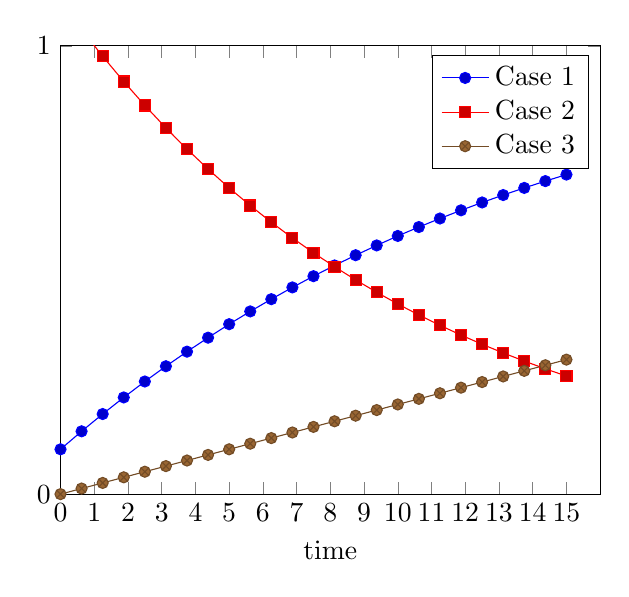
\begin{tikzpicture}
  \begin{axis}[ 
    xlabel= time,
    ylabel={},
    xtick = {0,1,2,3,4,5,6,7,8,9,10,11,12,13,14,15},
    ytick = {0,1},
    xmin = 0,
    ymin = 0,
    xmax = 16,
    ymax = 1,
    domain = 0:15
  ] 
    \addplot {1-((1.1^(-x))*(0.9+0.02*x))};
    \addplot {(1.1^(1-x))};
    \addplot {0.02*x};
    \legend{Case 1,Case 2, Case 3};
  \end{axis}
\end{tikzpicture}

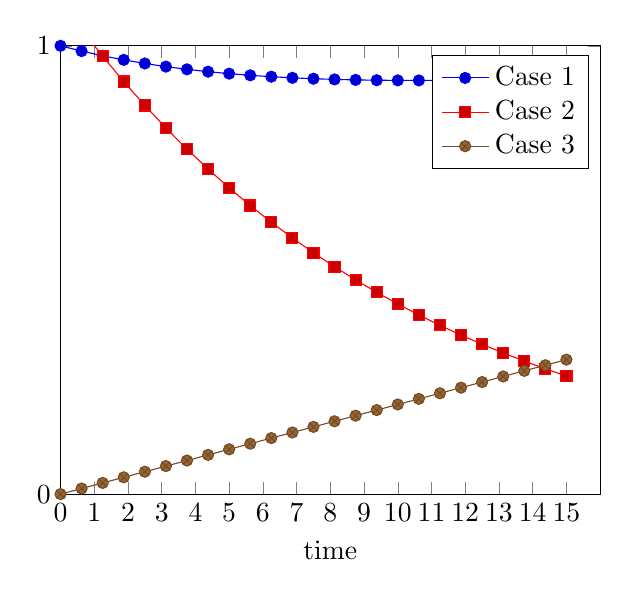
\begin{tikzpicture}
  \begin{axis}[ 
    xlabel= time,
    ylabel={},
    xtick = {0,1,2,3,4,5,6,7,8,9,10,11,12,13,14,15},
    ytick = {0,1},
    xmin = 0,
    ymin = 0,
    xmax = 16,
    ymax = 1,
    domain = 0:15
  ] 
    \addplot {1-((1.1^(-x))*(0.0+0.02*x))};
    \addplot {(1.1^(1-x))};
    \addplot {0.02*x};
    \legend{Case 1,Case 2, Case 3};
  \end{axis}
\end{tikzpicture}

\end{description} 

% \begin{thebibliography}{1}

%   \bibitem{notes} Pacheco, J.M., Santos, F.C., Souza, M.O. and Skyrms, B., {\em Evolutionary dynamics of collective action in N-person stag hunt dilemmas}  2009.

%   \bibitem{impj}  da Costa Ferreira, A.F., {\em DipBlue: a Diplomacy Agent with Strategic and Trust Reasoning} For Jury Evaluation.

% \end{thebibliography}

\bibliography{references}{}

\end{document}
